\documentclass[sigconf]{acmart}
% The preceding line is only needed to identify funding in the first footnote. If that is unneeded, please comment it out.
% On windows run updmap
\usepackage{color}
\usepackage{xcolor}
\usepackage{amsmath,amsfonts}
\usepackage{algorithmic}
\usepackage{graphicx}
\usepackage{textcomp}
\usepackage{listings}
\usepackage{multirow}
\usepackage{dcolumn}
\usepackage{booktabs} 
\usepackage{pifont}  % use /ding{55} for X... /ding{51} for check
\usepackage{adjustbox}
\usepackage{threeparttable}
\usepackage{hyperref}
\usepackage[nameinlink]{cleveref}
\usepackage{placeins}
\usepackage{subfig}


\expandafter\newcommand\csname r@tocindent4\endcsname{4in}
\setcounter{secnumdepth}{4}
\setcounter{tocdepth}{4}

\lstset{
language=Python,
basicstyle=\small\ttfamily,			
keywordstyle=\color{blue},
commentstyle=\color{gray},			
stringstyle=\color{black},					
}


\AtBeginDocument{%
  \providecommand\BibTeX{{%
    \normalfont B\kern-0.5em{\scshape i\kern-0.25em b}\kern-0.8em\TeX}}}

% My 'newcommand' for modulo function...



% My 'newcommand' for standard table creation...
\newcommand{\AndreaTable}[3]{\begin{table*}[h!]
\caption{#1}
\centering
\begin{tabular}{#2}
\toprule
#3
\bottomrule
\end{tabular}
\end{table*}
}

% My 'newcommand' for standard table creation...
\newcommand{\equivalenceClassesTable}[2]{
\AndreaTable{#1}{llm{8cm}m{8cm}}{#2}
}


\definecolor{beaublue}{rgb}{0.74, 0.83, 0.9}


\settopmatter{printacmref=false, printccs=false, printfolios =false}
\setcopyright{none} 
\renewcommand\footnotetextcopyrightpermission[1]{}
\acmConference[CPS Project A.A. 2020-2021]{ }{May 30, 2021}{ }

\begin{document}

\title{CPS Project A.A. 2020-2021}

\author{Andrea Graziani ($0273395$)}
\email{andrea.graziani93@outlook.it}
\affiliation{
  \institution{Università degli Studi di Roma "Tor Vergata"}
  \city{Rome}
  \country{Italy}
}

\maketitle


\newcommand{\AndreaCodeLink}[2]{\textcolor{blue}{\href{#1}{\texttt{\underline{#2}}}}}
\newcommand{\abs}[1]{\left|#1\right|}
\newcommand{\mathDef}{\overset{\textit{def}}{=}}



\section{Introduction}

In this report we will describe main data structures, classes and variables of our application, which can be used to manage several kind of \textbf{time series} data, plotting them and determining several useful informations according to our project's specification. 

Our application requires both Python \texttt{3.x}\footnote{\url{https://www.python.org/}} and \textit{Classic Jupyter Notebook}\footnote{\url{https://jupyter.org/}} to run properly, while, in order to perform the front-end rendering, \texttt{ipywidgets}\footnote{\url{https://ipywidgets.readthedocs.io/en/latest/}}, a python package containing several interactive HTML widgets for jupyter notebooks, is required. Anyhow, make sure you to satisfy all dependencies listed inside the \AndreaCodeLink{https://github.com/AndreaG93/CPS-Project/blob/main/README.md}{README} file before running this application on your system.

We remind that the source code of this application is available on \texttt{GitHub}\footnote{\url{https://github.com/AndreaG93/CPS-Project}}, including the \LaTeX\ source code of this report.

\section{Description}

\subsection{Jupyter Notebook Description}

In order to run the application, just run one of the \textit{two} code cell inside \texttt{CPS.ipynb} jupyter notebook file:

\begin{enumerate}
\item Running the first one, the user interface reported in \textbf{\cref{CodeCellOutput} (a)} will be shown and, using the interactive widgets displayed, you can plot a selected dataset applying various customizations.

From an implementation point of view, this user interference is provided by \AndreaCodeLink{https://github.com/AndreaG93/CPS-Project/blob/main/src/GUI/GUIPlot.py\#L6-L187}{GUIPlot} class which exports following methods: 

\begin{enumerate}
\item \AndreaCodeLink{https://github.com/AndreaG93/CPS-Project/blob/main/src/GUI/GUIPlot.py\#L42-L187}{\_\_build} method which includes all necessary code to instantiate all widgets including the so-called geometry management (that is where to put those widgets).

\item \AndreaCodeLink{https://github.com/AndreaG93/CPS-Project/blob/main/src/GUI/GUIPlot.py\#L35-L40}{display} method which, instead, is used to clean current jupyter notebook code cell and show all previously built widgets as output.
\end{enumerate}

\item Conversely, running the second code cell, will be displayed the user interface reported in \textbf{\cref{CodeCellOutput} (b)}, using which you can compare regression lines. 

This interface is built by \AndreaCodeLink{https://github.com/AndreaG93/CPS-Project/blob/main/src/GUI/GUIRegressionLineComparison.py}{GUIRegressionLineComparison} class which operates identically to \texttt{GUIPlot} class, despite it builds and manages different widgets.

\end{enumerate}

\begin{figure*}[h!]
    \centering
    \subfloat[\centering]{{\frame{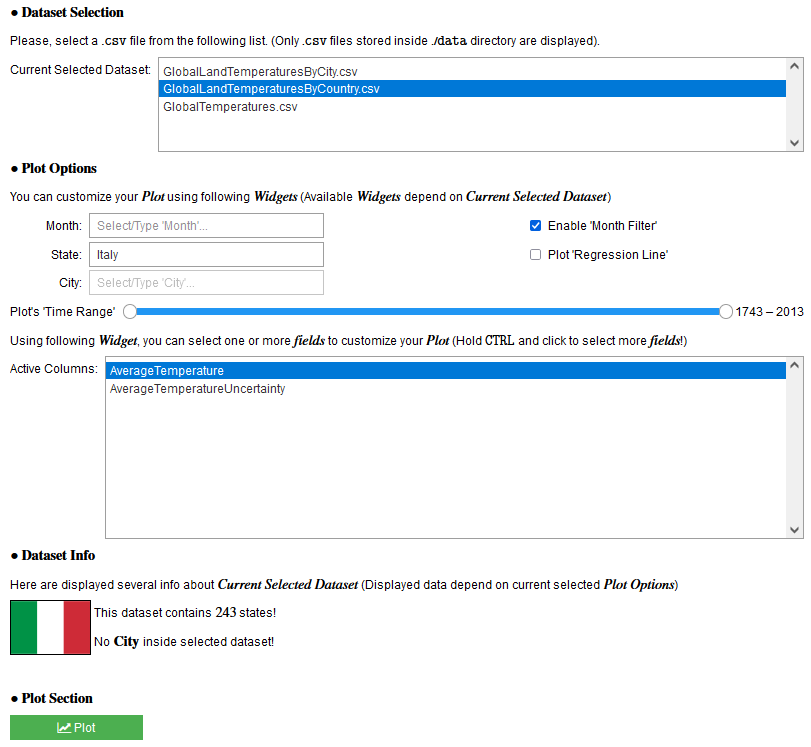
\includegraphics[width=8cm, height=6.5cm]{./screenshot/CodeCellOutput1.png}} }}%
    \qquad
    \subfloat[\centering]{{\frame{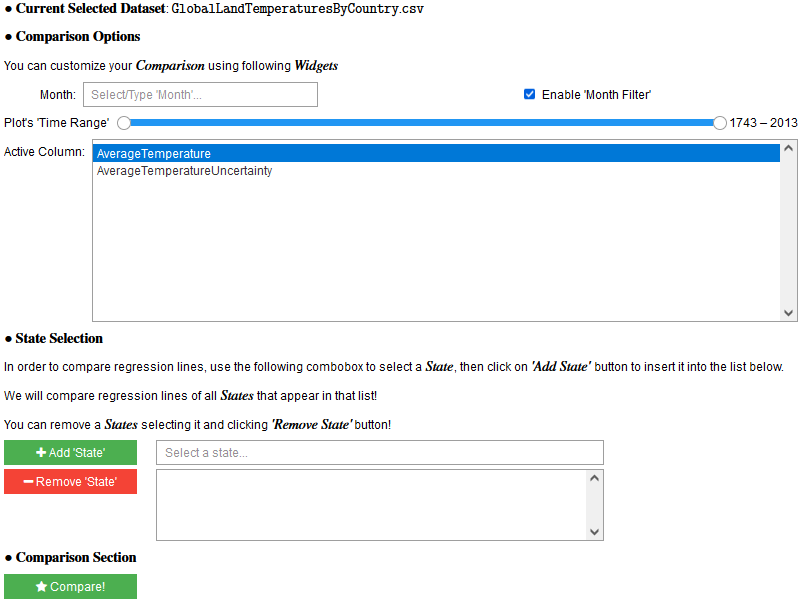
\includegraphics[width=8cm, height=6.5cm]{./screenshot/CodeCellOutput2.png}} }}%
    \caption{Application's GUI.}%
    \label{CodeCellOutput}%
\end{figure*}

To be precise, all tasks related to \textit{event handling}, \textit{widget callbacks function} and \textit{screen update} is managed by both \AndreaCodeLink{https://github.com/AndreaG93/CPS-Project/blob/main/src/GUI/GUIPlotController.py\#L11-L284}{GUIPlotController} and \AndreaCodeLink{https://github.com/AndreaG93/CPS-Project/blob/main/src/GUI/GUIRegressionLineComparisonController.py\#L10-L201}{GUIRegressionLineComparisonController} classes; however, we preferred to omit a detailed description of all classes involved into GUI rendering because they are just too technical and so not relevant for the purposes of this report. 

\subsection{\texttt{Application} Class Description}

However, to display any user interface, an instance of \AndreaCodeLink{https://github.com/AndreaG93/CPS-Project/blob/main/src/Application.py\#L23-L104}{Application} class is required.

From an architectural point of view, the \texttt{Application} class is used to model the internal state of our application, holding all references to available datasets and  plot customization options. To be more precise, this class has following responsibilities: 

\begin{itemize}
\item To instantiate and to maintain a reference to all \texttt{TimeSeries\-Data\-set} objects which, as explained later, are used to model all datasets.

This task can be done running \AndreaCodeLink{https://github.com/AndreaG93/CPS-Project/blob/main/src/Application.py\#L47-L74}{\_\_build\_dataset\_registry} method which firstly reads all \texttt{csv} files stored inside \texttt{/data} directory, then, after reading the header of datasets, instantiate the correct subclass of \texttt{TimeSeries\-Data\-set} class according to available columns inside the dataset itself. Do not worry, we will explain the characteristics of \texttt{TimeSeries\-Data\-set} class and of its subclasses later.

All instantiated \texttt{TimeSeries\-Data\-set} object are finally stored as \textit{key}-\textit{value} pair inside the dictionary \texttt{self.\_\_dataset\_registry}, where the \textit{key} is the file-name of corresponding dataset. 

\item To instantiate and to hold references to \AndreaCodeLink{https://github.com/AndreaG93/CPS-Project/blob/main/src/Application.py\#L5-L20}{ApplicationOptions} objects, which are used, instead, to store plots customization options, like \textit{time-range} or \textit{month filter}, specified by the user using the user interface.

This activity is performed running \AndreaCodeLink{https://github.com/AndreaG93/CPS-Project/blob/main/src/Application.py\#L76-L90}{\_\_\-build\_op\-tions\-\_re\-gistry}, which builds a \texttt{ApplicationOptions} object for each \texttt{TimeSeries\-Data\-set} object stored inside \texttt{self.\_\_dataset\_registry} field.

Similarly to the previous case, \texttt{ApplicationOptions} objects are stored into a dictionary data structure, using dataset file-name as keys.

\end{itemize}
  
\subsection{Datasets}

According to project's specification, we have used the datasets belonging to \textit{Global Climate Change Data}\footnote{You can download the dataset from: \url{https://data.world/data-society/global-climate-change-data}}, which include \textbf{time series data} where each instance, indexed by a \textit{time-stamp} represented by a string using the \texttt{ISO 8601} format \texttt{YYYY-MM-DD} without seconds, contains several observations about temperatures measured in several cities and states around the world.

Therefore, we have modelled aforementioned datasets using \AndreaCodeLink{https://github.com/AndreaG93/CPS-Project/blob/main/src/TimeSeriesDataset/TimeSeriesDataset.py\#L5-L62}{TimeSeriesDataset} class, whose responsibilities are:
\begin{enumerate}
\item Read data from file system running \AndreaCodeLink{https://github.com/AndreaG93/CPS-Project/blob/main/src/TimeSeriesDataset/TimeSeriesDataset.py\#L23-L32}{\_\_read\_data} method, returning a \texttt{pandas.DataFrame} object whose index is represented by \texttt{DatetimeIndex} object, obtained parsing time-stamps of the \texttt{dt} column inside the dataset file exploiting the \texttt{pandas.read\_csv} function.

\item Determine the time range of available data, which are needed to build the user interface, running \AndreaCodeLink{https://github.com/AndreaG93/CPS-Project/blob/main/src/TimeSeriesDataset/TimeSeriesDataset.py\#L34-L41}{\_\_com\-pu\-te\_\-ti\-me\_range}.

\item Determine which columns contain numeric data running \AndreaCodeLink{https://github.com/AndreaG93/CPS-Project/blob/main/src/TimeSeriesDataset/TimeSeriesDataset.py\#L43-L47}{\_\_compute\_numeric\_type\_columns}.
\end{enumerate}

\subsection{Datasets Files}

Respecting project's specifications, our application is capable to manage following datasets files:

\begin{description}
\item[\texttt{GlobalLandTemperaturesByCity.csv}] This dataset includes the observations of \textit{Average Temperature} and \textit{Average Temperature Uncertainty}, collected from \textit{1743-11-01} to \textit{2013-09-01}, regarding several \textit{states} and \textit{cities} of the world.

From an implementation point of view, this dataset is represented by \AndreaCodeLink{https://github.com/AndreaG93/CPS-Project/blob/main/src/TimeSeriesDataset/TimeSeriesDatasetGlobalClimateChange.py\#L11-L220}{TimeSeriesDatasetGlobalClimateChange} class, a subclass of \texttt{TimeSeriesDataset}. 

This class exports several methods used to manage all data regarding states and cities of all available observations, reading data from \texttt{country} and \texttt{city} columns inside the dataset file.

For example, \AndreaCodeLink{https://github.com/AndreaG93/CPS-Project/blob/main/src/TimeSeriesDataset/TimeSeriesDatasetGlobalClimateChange.py\#L32-L39}{get\_state\_list} and
\AndreaCodeLink{https://github.com/AndreaG93/CPS-Project/blob/main/src/TimeSeriesDataset/TimeSeriesDatasetGlobalClimateChange.py\#L41-L48}{get\_city\_list} methods are used to compute a list of all available states and cities respectively inside the dataset.
 
Conversely, \AndreaCodeLink{https://github.com/AndreaG93/CPS-Project/blob/main/src/TimeSeriesDataset/TimeSeriesDatasetGlobalClimateChange.py\#L50-L63}{get\_city\_list\_belonging\_to\_state} method is used to determine all cities belonging to a specified state. Moreover, this class exports the \AndreaCodeLink{https://github.com/AndreaG93/CPS-Project/blob/main/src/TimeSeriesDataset/TimeSeriesDatasetGlobalClimateChange.py\#L65-L79}{get\_state\_of\_city} method, which can be used to know the state to which a specified city belongs.

Please note that, in order to save computing resources by avoiding unneeded computations, all informations about cities and states are computed exploiting \textit{lazy evaluation}, that is aforementioned data are evaluated only on the first need and stored them in case they would be needed again later.

\item[\texttt{GlobalLandTemperaturesByCountry.csv}] This dataset is similar to the previous one except for the absence of \texttt{city} column, therefore \AndreaCodeLink{https://github.com/AndreaG93/CPS-Project/blob/main/src/TimeSeriesDataset/TimeSeriesDatasetGlobalClimateChange.py\#L225-L241}{TimeSeriesDatasetGlobalClimate\-Change\-NoCity} class was used to model this dataset. Observe that it is a subclass of \texttt{TimeSeriesDatasetGlobalClimateChange} and, as you can see from code, to reflect the absence of data about cities, we have performed method overriding accordingly.

\item[\texttt{GlobalLandTemperatures.csv}] This dataset includes data from \textit{1750-01-01} to \textit{2015-12-01} regarding several kinds of observations like \textit{Land Average Temperature}, \textit{Land Average Temperature Uncertainty} and so on.

Since this dataset file contains neither \texttt{country} and \texttt{city} columns, \AndreaCodeLink{https://github.com/AndreaG93/CPS-Project/blob/main/src/TimeSeriesDataset/TimeSeriesDatasetGlobalClimateChange.py\#L244-L263}{TimeSeriesDatasetGlobalClimateChangeNoStateNoCity} class was been used and, like previously, we have performed method overriding accordingly to the characteristics of this dataset.

\end{description}

\subsection{The \textit{Datasets Info} and \textit{Plot Options} sections}

All aforementioned methods are used to properly manage the user interface, setting and updating the contents of all widgets inside the "\textit{Plot Options}" section of the GUI (see \textbf{\cref{CodeCellOutput} (a)}); for example, \texttt{get\_state\_list} and \texttt{get\_city\_list} methods are used to populate available choices of both "\textit{State}" and "\textit{City}" combo-box widgets.

However, \texttt{TimeSeriesDatasetGlobalClimateChange} class methods allow us to determine several informations about a selected dataset too. 

In fact, application's user interface provides another section, called "\textit{Dataset Info}", where following information are displayed to the user when a dataset, equipped with both \texttt{country} and \texttt{city} columns, is selected:

\begin{enumerate}
\item The total number of states or nations represented inside current selected dataset.
\item The total number of cities available inside the entire current selected dataset.
\end{enumerate}

Moreover, according to project's specification, after selecting a state will be displayed the number of cities belonging to it.

For example, if you select \texttt{GlobalLandTemperaturesByCity.csv} dataset specifying \textit{Italy} as selected state, the output, reported in \textbf{\cref{DatasetInfo}}, will be shown. 

\begin{figure}
    \frame{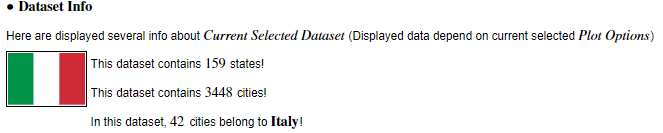
\includegraphics[width=8cm]{./screenshot/DatasetInfo.png}}
    \caption{An example of \textit{Dataset info} section output}%
    \label{DatasetInfo}%
\end{figure}

Furthermore, using \texttt{get\_city\_list\_belonging\_to\_state} method, is very simple to know which cities belongs to a selected state and select it in order to customize your plot. \textbf{\cref{ItalianCombobox}} shows the output displayed when \textit{Italy} state is set and \textit{City} combo-box is selected.

\begin{figure}[h]
    \frame{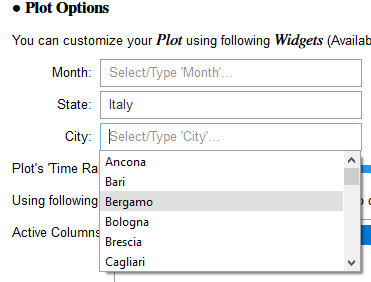
\includegraphics[width=8cm]{./screenshot/CityCombobox.png}}
    \caption{The City Combo-box displaying only Italian cities.}%
    \label{ItalianCombobox}%
\end{figure}

The flag of the selected state, displayed inside "\textit{Datasets Info}" section, is retrieved exploiting \texttt{RESTful API} belonging to a provider called \texttt{REST COUNTRIES}\footnote{\url{https://restcountries.eu/}}. 

From an implementation point of view, all requests are forwarded using \AndreaCodeLink{https://github.com/AndreaG93/CPS-Project/blob/main/src/GUI/RestAPI/StateFlagUrlRegistry.py\#L35-L53}{\_\_get\_url\_from\_rest\_api} static method, implemented inside \AndreaCodeLink{https://github.com/AndreaG93/CPS-Project/blob/main/src/GUI/RestAPI/StateFlagUrlRegistry.py\#L5-L57}{StateFlagUrlRegistry} class whose structure is based on so-called \textit{registry design pattern}, which was been adopted to simplify the storing and the retrieving of state flags without forwarding unneeded requests.

\subsection{Plot}

When you will finish to set all needed plot customization options, you can plot your data clicking the button "\textit{Plot}" displayed inside "\textit{Plot Section}". The click event triggers the invocation of \AndreaCodeLink{https://github.com/AndreaG93/CPS-Project/blob/main/src/GUI/GUIPlotController.py\#L36-L104}{plot\_event} method which manages all tasks necessary for plotting data. 

The most important work is done by \AndreaCodeLink{https://github.com/AndreaG93/CPS-Project/blob/main/src/TimeSeriesDataset/TimeSeriesDatasetGlobalClimateChange.py\#L81-L193}{get\_filtered\_data} method exported by \texttt{TimeSeriesDatasetGlobalClimateChange} class, which includes all application logic used to perform following tasks:
\begin{enumerate}
\item apply plot customization options to selected data, which is done exploiting \texttt{pandas} python package.
\item check correctness of user input.
\item pre-process data, looking for missing records and \texttt{NaN} values. 

This activity is done exploiting \texttt{pandas.DataFrame.reindex}\footnote{\url{https://pandas.pydata.org/pandas-docs/stable/reference/api/pandas.DataFrame.reindex.html}} method, according to which the \texttt{DataFrame} object is conformed to new index built using \texttt{pandas.date\_range}\footnote{\url{https://pandas.pydata.org/pandas-docs/stable/reference/api/pandas.date\_range.html}} method using a \textit{sampling frequency} (the number of sampling points per unit time) equal to that of the dataset, which is equal at one data point every first day of every month. 

In this way, we are able to find missing records which, according to our experiments, are present inside every dataset\footnote{Please note that the number of missing records is suppressed by default; however, you can print it de-commenting some line of code inside \texttt{get\_filtered\_data} method.}.

Finally, to manage \texttt{NaN} values, we have simply exploited \texttt{interpolate}\footnote{\url{https://pandas.pydata.org/pandas-docs/stable/reference/api/pandas.DataFrame.interpolate.html}} and \texttt{dropna}\footnote{\url{https://pandas.pydata.org/pandas-docs/stable/reference/api/pandas.DataFrame.dropna.html}} functions.
\end{enumerate}

Finally, invoking \AndreaCodeLink{https://github.com/AndreaG93/CPS-Project/blob/main/src/Common.py\#L32-L48}{plot} function, the plot will be displayed like in \textbf{\cref{PlotExample}}, inside which a regression line is displayed too.

\begin{figure}[h]
    \frame{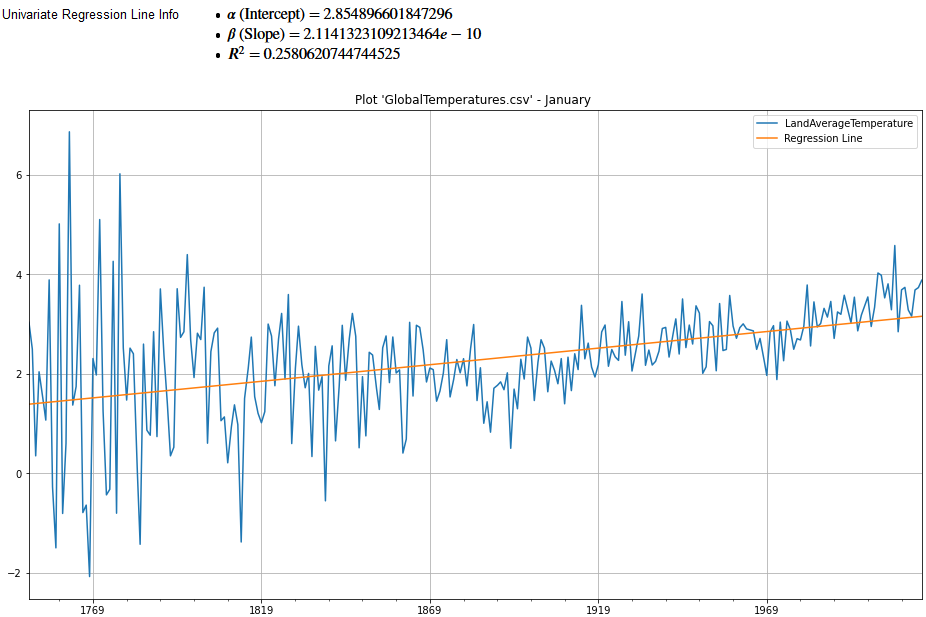
\includegraphics[width=8cm]{./screenshot/ExamplePlot.png}}
    \caption{Output plot}%
    \label{PlotExample}%
\end{figure}

\section{Regression Line Computation}

In this last section, we will describe how a regression line is computed.

\subsection{\texttt{SimpleRandomSample} Class Description}

The \AndreaCodeLink{https://github.com/AndreaG93/CPS-Project/blob/main/src/Statistics/SimpleRandomSample.py\#L1-L76}{SimpleRandomSample} class is used to model a \textbf{random sample} holding the values $x_1,x_2,...,x_n$ of a random sample $X_1,X_2,...,X_n$ of size $n \in \mathbb{N}$, where $X_1,X_2,...,X_n$ are \textit{independent random variables} that satisfy following equation:

\begin{equation}
X \overset{\mathrm{\textit{d}}}{=} X\qquad \forall k = 1,...,n
\end{equation}

that is, $X_1,X_2,...,X_n$ converge in distribution to a real random variable $X$.

This class allows us to compute following \textit{statistics} of a given random sample:
\begin{description}

\item[Sample Mean] which is computed by \AndreaCodeLink{https://github.com/AndreaG93/CPS-Project/blob/main/src/Statistics/SimpleRandomSample.py\#L17-L29}{get\_mean} function using following formula:
\begin{equation}
\overline{x}_n \mathDef \frac{1}{n}\sum_{k=1}^n x_k
\end{equation}

\item[Unbiased Sample Variance] which is determined exploiting \AndreaCodeLink{https://github.com/AndreaG93/CPS-Project/blob/main/src/Statistics/SimpleRandomSample.py\#L31-L43}{get\_unbiased\_variance} function using following equation:
\begin{equation}
s^2_n(X) \mathDef \frac{1}{n-1}\sum_{k=1}^n (x_k - \overline{x}_n)^2
\end{equation}

\item[Sample Covariance] which is, instead, provided by a static method, called \AndreaCodeLink{https://github.com/AndreaG93/CPS-Project/blob/main/src/Statistics/SimpleRandomSample.py\#L51-L76}{calc\_sample\_covariance}, using following equation:

\begin{equation}
s_n(X,Y) \mathDef \frac{1}{n-1}\sum_{k=1}^n (x_k - \overline{x}_n)(y_k - \overline{y}_n)
\end{equation}

\end{description}

\subsection{\texttt{UnivariateRegressionLine} Class Description}

All statistics computed by a \texttt{SimpleRandomSample} instance are used to compute regression lines, which are been modelled using \AndreaCodeLink{https://github.com/AndreaG93/CPS-Project/blob/main/src/Statistics/UnivariateRegressionLine.py\#L4-L117}{UnivariateRegressionLine} class.

To be more precise, that class holds all data needed to represent a \textit{linear regression function} $f : \mathbb{R} \times \mathbb{R}^2 \longrightarrow \mathbb{R}$ given by:

\begin{equation}
f(x; \theta) \overset{\mathrm{\textit{def}}}{=} \alpha + \beta x \qquad \forall x \in \mathbb{R}
\end{equation}

where $\theta \equiv (\alpha , \beta) \in \mathbb{R}^2$ is the \textit{regression parameter}, where $\alpha$ is called \textit{intercept} while $\beta$ is knowns as \textit{slope}.

Regression parameter is computed by \AndreaCodeLink{https://github.com/AndreaG93/CPS-Project/blob/main/src/Statistics/UnivariateRegressionLine.py\#L37-L45}{\_\_calc\_slope\_and\_intercept} method, using following equations:

\begin{equation}
\alpha = \overline{y}_n - \beta \overline{x}_n \qquad \beta = \dfrac{s_n(X,Y)}{s^2_n(X)}
\end{equation}

Then, all points of the regression line $(x_k,\hat{y}_k)_{k=1}^n$ are computed by \AndreaCodeLink{https://github.com/AndreaG93/CPS-Project/blob/main/src/Statistics/UnivariateRegressionLine.py\#L46-L53}{\_\_calc\_fitted\_values} method using following equation:

\begin{equation}
\hat{y}_k \mathDef \alpha + \beta x_k \qquad \forall k = 1,2,...,n
\end{equation}

From an implementation point of view, the regression line is computed running \AndreaCodeLink{https://github.com/AndreaG93/CPS-Project/blob/main/src/TimeSeriesDataset/TimeSeriesDatasetGlobalClimateChange.py\#L193-L208}{compute\_univariate\_regression\_line} function.
 
However, \texttt{UnivariateRegressionLine} class has another very important responsibility: to perform regression lines comparison tasks.

Regression lines comparison is needed to determine which state, belonging to a previously user defined list, has the \textit{worst} regression line in a specified time range. 
To perform this task, we exploited the \textit{coefficient of determination}, also denoted $R^2$, which is the positive number defined as follows:

\begin{equation}
R^2 \mathDef \dfrac{ESS}{TSS}
\end{equation}

where $ESS$ is the so-called \textit{explained sum of squares} while $TSS$ is the \textit{total sum of squares}, which are computed by \AndreaCodeLink{https://github.com/AndreaG93/CPS-Project/blob/main/src/Statistics/UnivariateRegressionLine.py\#L61-L67}{\_\_calc\_ess} and \AndreaCodeLink{https://github.com/AndreaG93/CPS-Project/blob/main/src/Statistics/UnivariateRegressionLine.py\#L54-L60}{\_\_calc\_tss} respectively, using following equations:

\begin{equation}
ESS \mathDef \sum_{k=1}^n (\hat{y}_k - \overline{y}_n)^2 \qquad TSS \mathDef \sum_{k=1}^n (y_k - \overline{y}_n)^2
\end{equation}

The $R^2$ value is very useful because tell us how much the fitted/predicted data $\hat{y}$, explains the actual data $y$. In particular, the higher the value of $R^2$ the more successfully the variation in the data set $(y_k)^k_{n=1}$ can be explained in terms of the linear dependence on the data set $(x_k)^k_{n=1}$ expressed by the regression
line. The $R^2$ value ranges from $0$ to $1$, with higher values denoting a strong fit, and lower values denoting a weak fit.

To perform this task, we exploited \AndreaCodeLink{https://github.com/AndreaG93/CPS-Project/blob/main/src/GUI/GUIPlot.py\#L103-L120}{rank\_regression\_lines} static method defined inside \texttt{UnivariateRegressionLine} class. After the comparison of regression lines, as you can see from the example reported in \textbf{\cref{ExampleComparison}}, will be finally displayed as output a rank of regression lines based on best $R^2$ values printing which state has the worst regression line.

\begin{figure}
    \frame{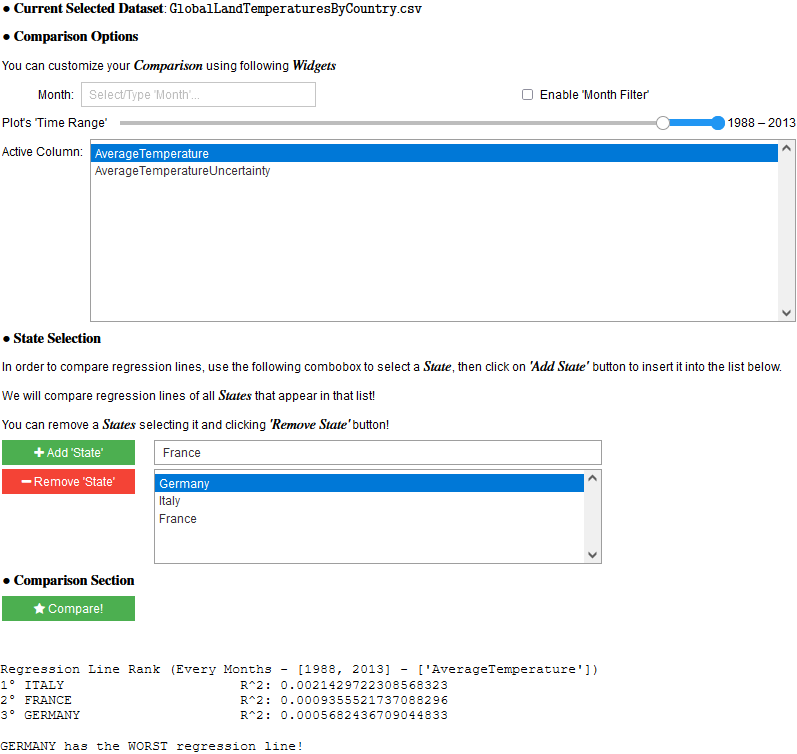
\includegraphics[width=9cm]{./screenshot/ExampleComparison.png}}
    \caption{Which country between \textit{Italy}, \textit{France} and \textit{Germany} has the \textit{worst} regression line in the last 25 years?}%
    \label{ExampleComparison}%
\end{figure}


\FloatBarrier


\end{document}
\endinput







